\section{Introduction to the Course}
\begin{frame}{What Is Image Processing?}
    \begin{itemize}%[<+->]
        \item In digital image processing, we manipulate a digital image to produce another digital image, which is an enhanced version of the original image.
        \item E.g., blurring, noise filtering, color enhancement, segmentation (?).
    \end{itemize}

    \begin{figure}[ht]
      \centering
      \begin{subfigure}[b]{0.5\linewidth}
        \centering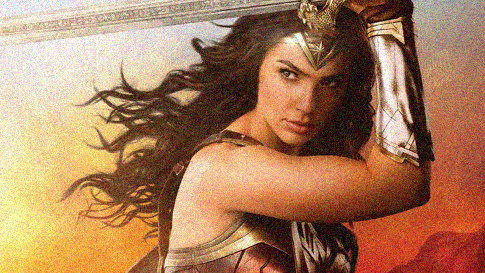
\includegraphics[width=100pt]{galn.png}
        \caption{Noisy image}\label{sf:galn}
      \end{subfigure}%
      \begin{subfigure}[b]{0.5\linewidth}
        \centering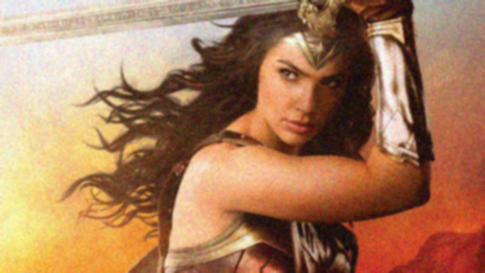
\includegraphics[width=100pt]{galb.png}
        \caption{Gaussian filtered image}\label{sf:galb}
      \end{subfigure}\\
      \begin{subfigure}[b]{0.5\linewidth}
        \centering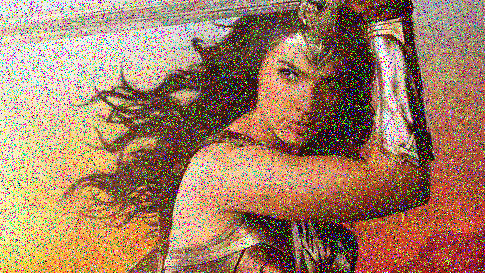
\includegraphics[width=100pt]{gals.png}
        \caption{Image with salt and pepper noise}\label{sf:gals}
      \end{subfigure}%
      \begin{subfigure}[b]{0.5\linewidth}
        \centering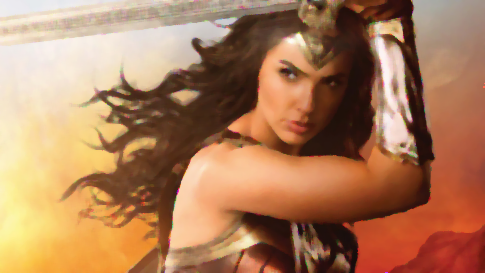
\includegraphics[width=100pt]{galm.png}
        \caption{Median filtered image}\label{sf:galm}
      \end{subfigure}
      \caption{Filtering}
    \end{figure}
\end{frame}

\begin{frame}{What is computer vision?}
    \begin{itemize}%[<+->]
        \item In computer vinson, we analyze a digital images or videos  to  make a decision.
        \item E.g., face detection, object detection, semantic segmentation.
    \end{itemize}
    \begin{figure}[ht]
      \centering
      \begin{subfigure}[b]{0.5\linewidth}
        \centering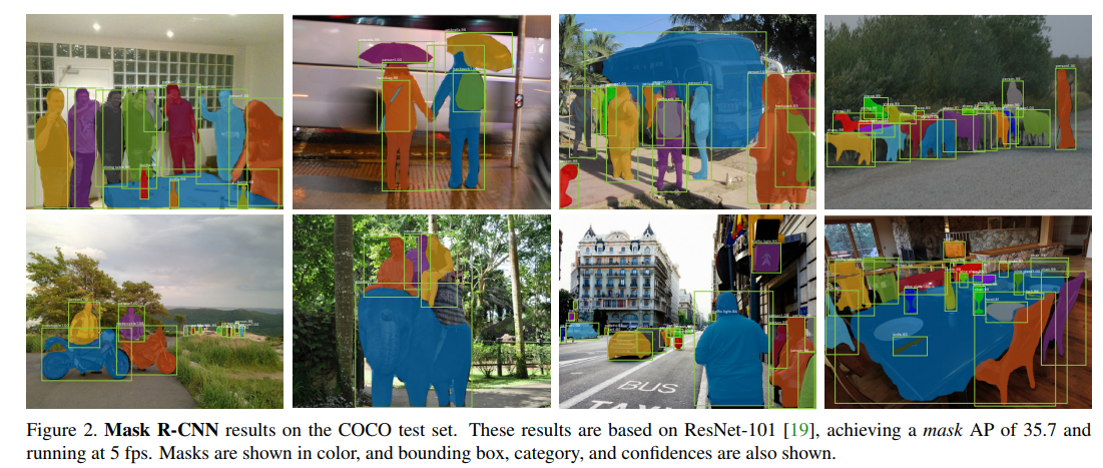
\includegraphics[width=100pt]{mask_rcnn.png}
        \caption{Mask RCNN Object detection and semantic segmentation}\label{sf:mask_rc}
      \end{subfigure}%
      \begin{subfigure}[b]{0.5\linewidth}
        \centering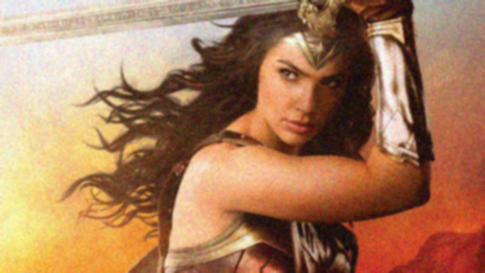
\includegraphics[width=100pt]{galb.png}
        \caption{Gaussian filtered image}\label{sf:galb}
      \end{subfigure}\\
      \caption{Examples of computer vsion.}
    \end{figure}
\end{frame}

\begin{frame}{Text Books}
    \begin{enumerate}
        \item Gonzalez and Woods, Digital Image Processing
        \item Forsyth and Ponce, Computer Vision: A Modern Approach
        \item Richard Szeliski, Computer Vision: Algorithms and Applications (available online)
        \item Milan Sonka, Image Processing, Analysis, and Machine Vision
    \end{enumerate}
    \begin{figure}[ht]
      \centering
      \begin{subfigure}[b]{0.22\linewidth}
        \centering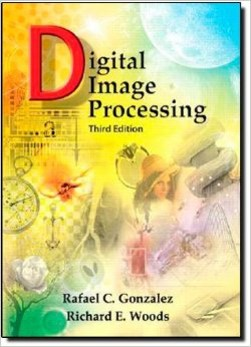
\includegraphics[width=50pt]{gw.jpg}
        \caption{}\label{sf:gw}
      \end{subfigure}%
      \begin{subfigure}[b]{0.22\linewidth}
        \centering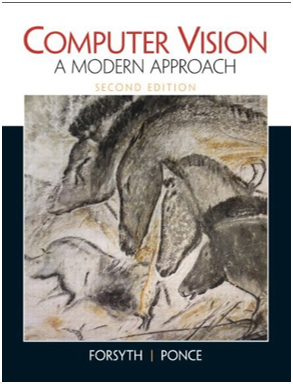
\includegraphics[width=50pt]{fp.png}
        \caption{}\label{sf:fp}
      \end{subfigure}
      \begin{subfigure}[b]{0.22\linewidth}
        \centering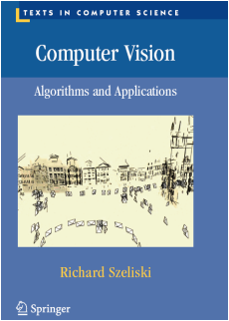
\includegraphics[width=50pt]{rz.png}
        \caption{}\label{sf:rz}
      \end{subfigure}
      \begin{subfigure}[b]{0.22\linewidth}
        \centering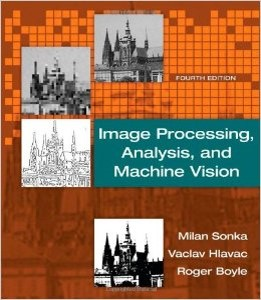
\includegraphics[width=50pt]{ms.jpg}
        \caption{}\label{sf:ms}
      \end{subfigure}
      \caption{}
    \end{figure}

\end{frame}

\begin{frame}{Course Requirements}
    \begin{enumerate}
        \item Programming assignments: 20\%
        \item Four assignments
        \begin{itemize}
            \item Expect the first one in the next couple of classes.
            \item We use OpenCV and Python. Revise your Python and Numpy knowledge.
            \item Other platforms,  e.g., MATLAB or OpenCV withe C++, are fine too.
        \end{itemize}
        \item Grading
        \begin{tabular}{@{}llccr@{}}
          \toprule
          Item   & Date& Weight& Minimum& Comments\\
          \midrule
          In-class quizzes &  Surprise & 5\% & 50\%& Easy\\
          \hline
          Assignment 1 &  To be scheduled & 5\% & 50\%& Easy\\
          \hline
          Assignment 2 & To be scheduled 9& 5\% & 50\%& Easy\\
          \hline
          Assignment 3&  To be scheduled&5\% & 50\%& Moderately difficult\\
          \hline
          Assignment 4&  To be scheduled &10\% & 50\%& Moderately difficult\\
          \hline
          Final examination & To be scheduled & 70\% & 50\%&?\\
          \bottomrule
        \end{tabular}
    \end{enumerate}
\end{frame}


\begin{frame}{Tips for Successful Completion}
    To extract meaning from pixels.
    \begin{enumerate}
      \item Mindset: ``I want to solve this vision problem. What are the tools available? How have others solved it? How should I go about solving it?''
      \item Attend every single lecture.
      \item Go through the material the night before and engage in a good discussion in class.
      \item Implement at least one algorithm discussed in class before the next class. This is in addition to the assignments.
    \end{enumerate}
\end{frame}

\begin{frame}{Academic Integrity Policy}
    \begin{itemize}
      \item You may discuss the assignments with each other. However, you must code on your own, and make the submissions on your own.
      \item You may benefit from the code and information on the internet, as long as you do not borrow code for the main theme of the assignment.
      \item Acknowledge  your sources.
    \end{itemize}
    \vfill
    \scriptsize{Source: S. Lazebnik}
\end{frame}

\begin{frame}{The Goal of Computer Vision}
    \begin{figure}[ht]
      \centering
      \begin{subfigure}[b]{0.5\linewidth}
        \centering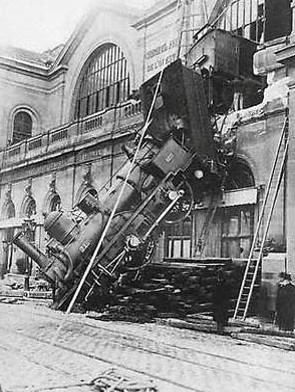
\includegraphics[width=100pt]{gare_montparnasse.jpg}
        \caption{What we see.}\label{sf:gare_montparnasse}
      \end{subfigure}%
      \begin{subfigure}[b]{0.5\linewidth}
        \centering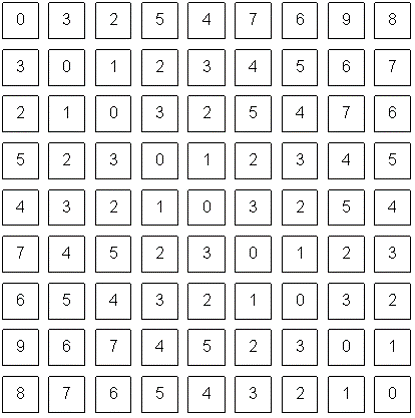
\includegraphics[width=100pt]{computer_view.png}
        \caption{What computer sees.}\label{sf:computer_view}
      \end{subfigure}
    \end{figure}
    \vfill
    \scriptsize{Source: S. Narasimhan}
\end{frame}

\section{Sate-of-the-Art in Vision}

\begin{frame}{Reconstruction: 3D from Photo Collections}
    \begin{figure}[ht]
        \centering
        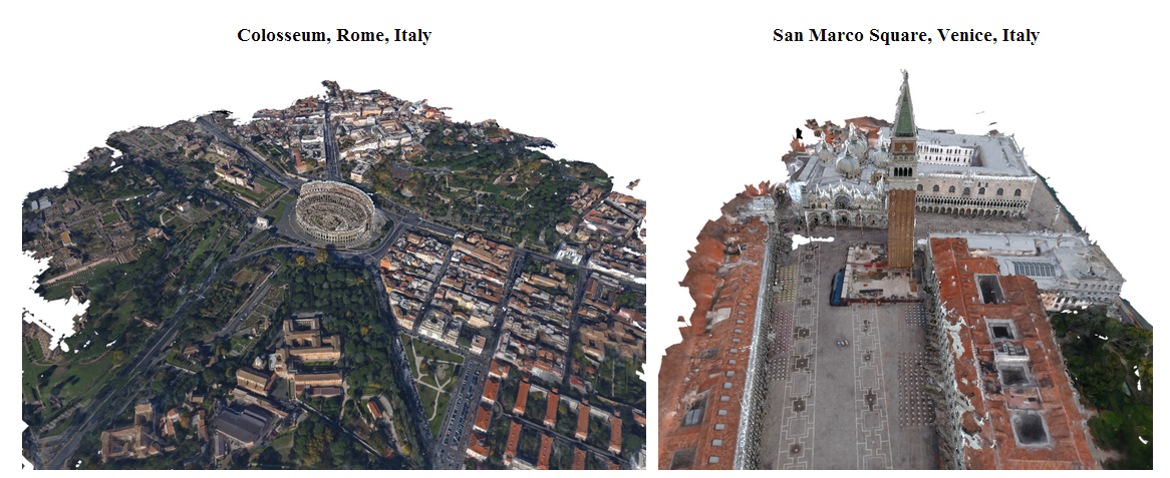
\includegraphics[width=10cm]{visual_turing.png}
        %\caption{What we see.}\label{fi:visual_turing}
    \end{figure}
    Q. Shan, R. Adams, B. Curless, Y. Furukawa, and S. Seitz, The Visual Turing Test for Scene Reconstruction, 3DV 2013.
    \url{https://www.youtube.com/watch?v=NdeD4cjLI0c}
    \vfill
    \scriptsize{Source: S. Lazebnik}
\end{frame}

\begin{frame}{Reconstruction: 4D from Photo Collections}
    \begin{figure}[ht]
        \centering
        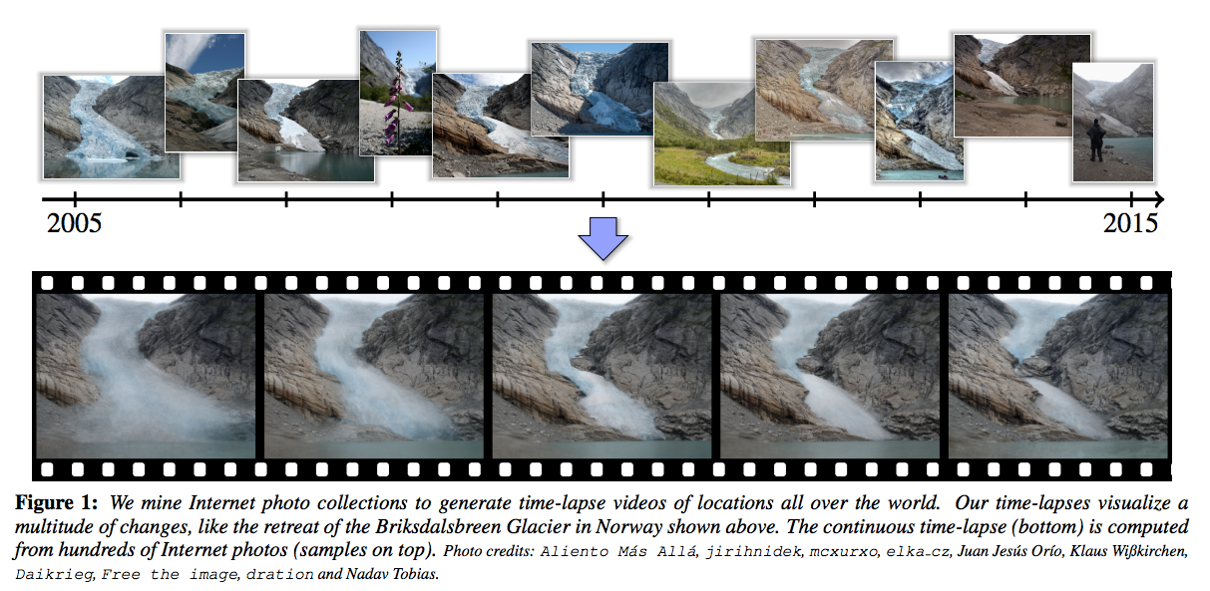
\includegraphics[width=10cm]{photos_to_4d.png}
    \end{figure}
    R. Martin-Brualla, D. Gallup, and S. Seitz, Time-Lapse Mining from Internet Photos, SIGGRAPH 2015.
    \url{https://www.youtube.com/watch?v=wptzVm0tngc&feature=youtu.be}
    \vfill
    \scriptsize{Source: S. Lazebnik}
\end{frame}

\begin{frame}{Reconstruction: 4D from Depth Cameras}
    \begin{figure}[ht]
        \centering
        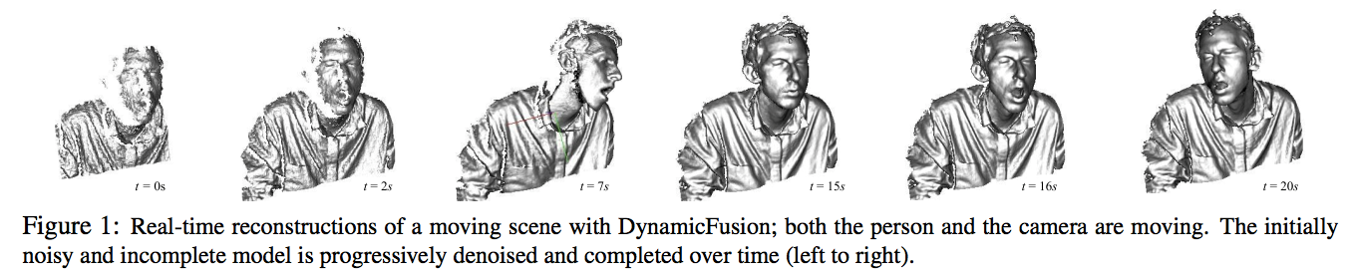
\includegraphics[width=10cm]{depth_to_4d.png}
    \end{figure}
    R. Newcombe, D. Fox, and S. Seitz, DynamicFusion: Reconstruction and Tracking of Non-rigid Scenes in Real-Time, CVPR 2015.
    \url{https://www.youtube.com/watch?v=i1eZekcc\_lM&feature=youtu.bee}
    \vfill
    \scriptsize{Source: S. Lazebnik}
\end{frame}


\begin{frame}{Reconstruction in Construction Industry}
    \begin{figure}[ht]
        \centering
        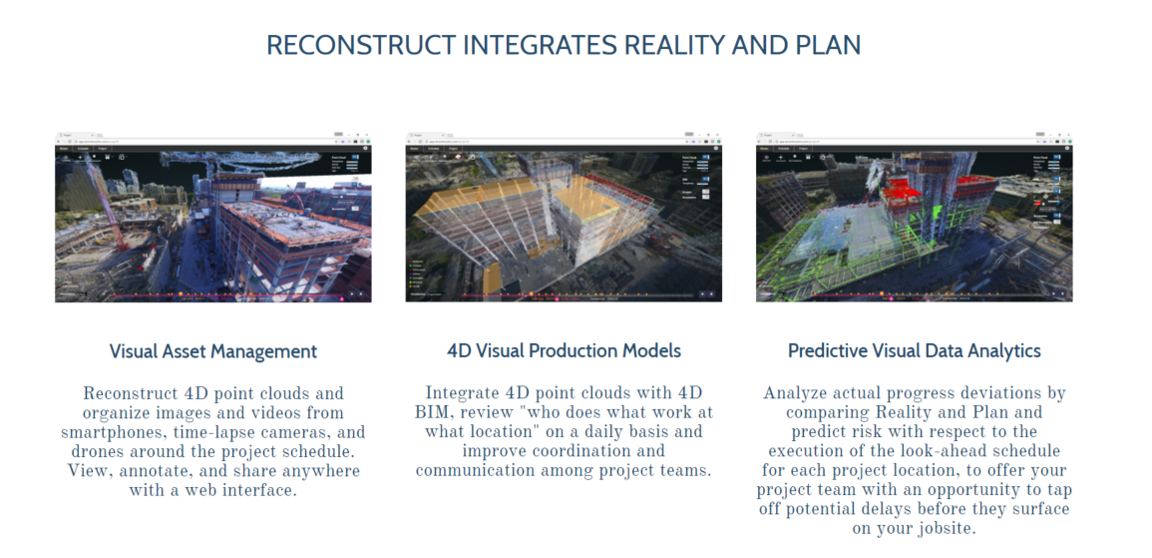
\includegraphics[width=10cm]{construction_industry}
    \end{figure}
    \url{https://www.reconstructinc.com/\#product-demo}
    \vfill
    \scriptsize{Source: D. Hoiem}
\end{frame}



\begin{frame}{Recognition: ``Simple Patterns''}
    \begin{figure}[ht]
      \centering
      \begin{subfigure}[b]{0.45\linewidth}
        \centering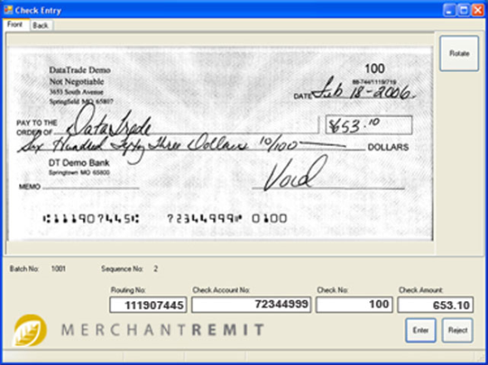
\includegraphics[width=100pt]{cheque.png}
        \caption{}\label{sf:cheque}
      \end{subfigure}%
      \begin{subfigure}[b]{0.45\linewidth}
        \centering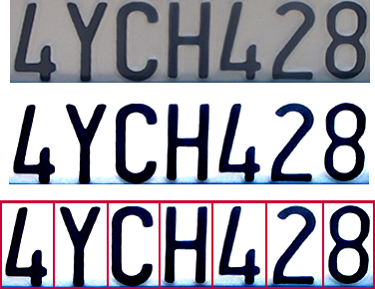
\includegraphics[width=100pt]{lpr.png}
        \caption{}\label{sf:lpr}
      \end{subfigure}\\
      \begin{subfigure}[b]{0.45\linewidth}
        \centering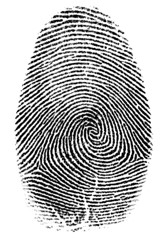
\includegraphics[width=50pt]{finger_print.jpg}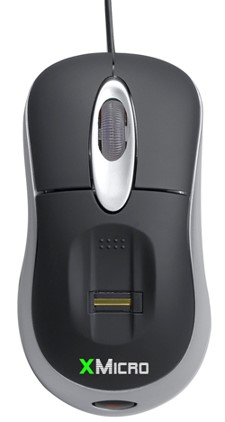
\includegraphics[width=50pt]{mouse.jpg}
        \caption{}\label{sf:mouse}
      \end{subfigure}
      \begin{subfigure}[b]{0.45\linewidth}
        \centering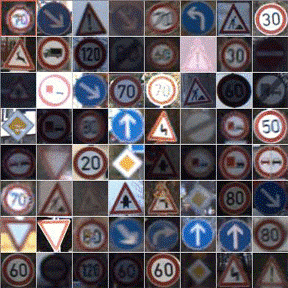
\includegraphics[width=100pt]{road_sign.png}
        \caption{}\label{sf:sign}
      \end{subfigure}
      \caption{}
    \end{figure}
\end{frame}



\begin{frame}{Recognition: Faces}
    \begin{figure}[ht]
      \centering
      \begin{subfigure}[b]{0.45\linewidth}
        \centering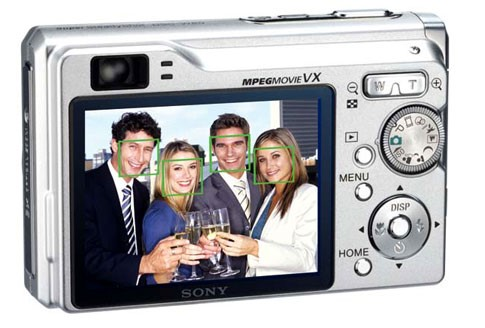
\includegraphics[width=100pt]{digital_cameras.jpg}
        \caption{}\label{sf:digital_cameras}
      \end{subfigure}%
      \begin{subfigure}[b]{0.45\linewidth}
        \centering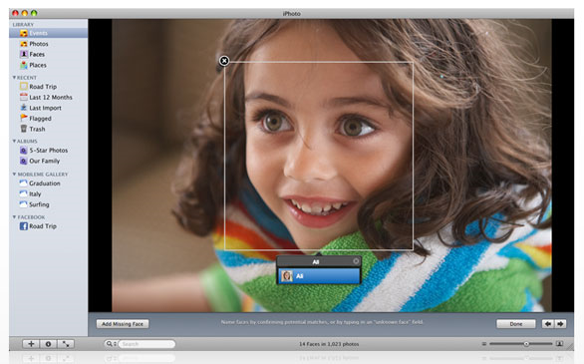
\includegraphics[width=100pt]{fr_software.png}
        \caption{}\label{sf:fr_software}
      \end{subfigure}\\
      \begin{subfigure}[b]{0.45\linewidth}
        \centering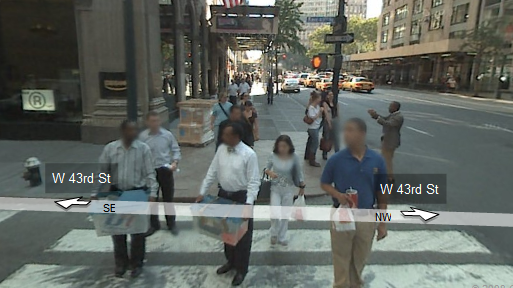
\includegraphics[width=100pt]{fr_blurr.png}
        \caption{}\label{sf:fr_blurr}
      \end{subfigure}
      \caption{}
    \end{figure}
\end{frame}



\begin{frame}{Concerns about Face Recognition}
    \begin{figure}[ht]
        \centering
        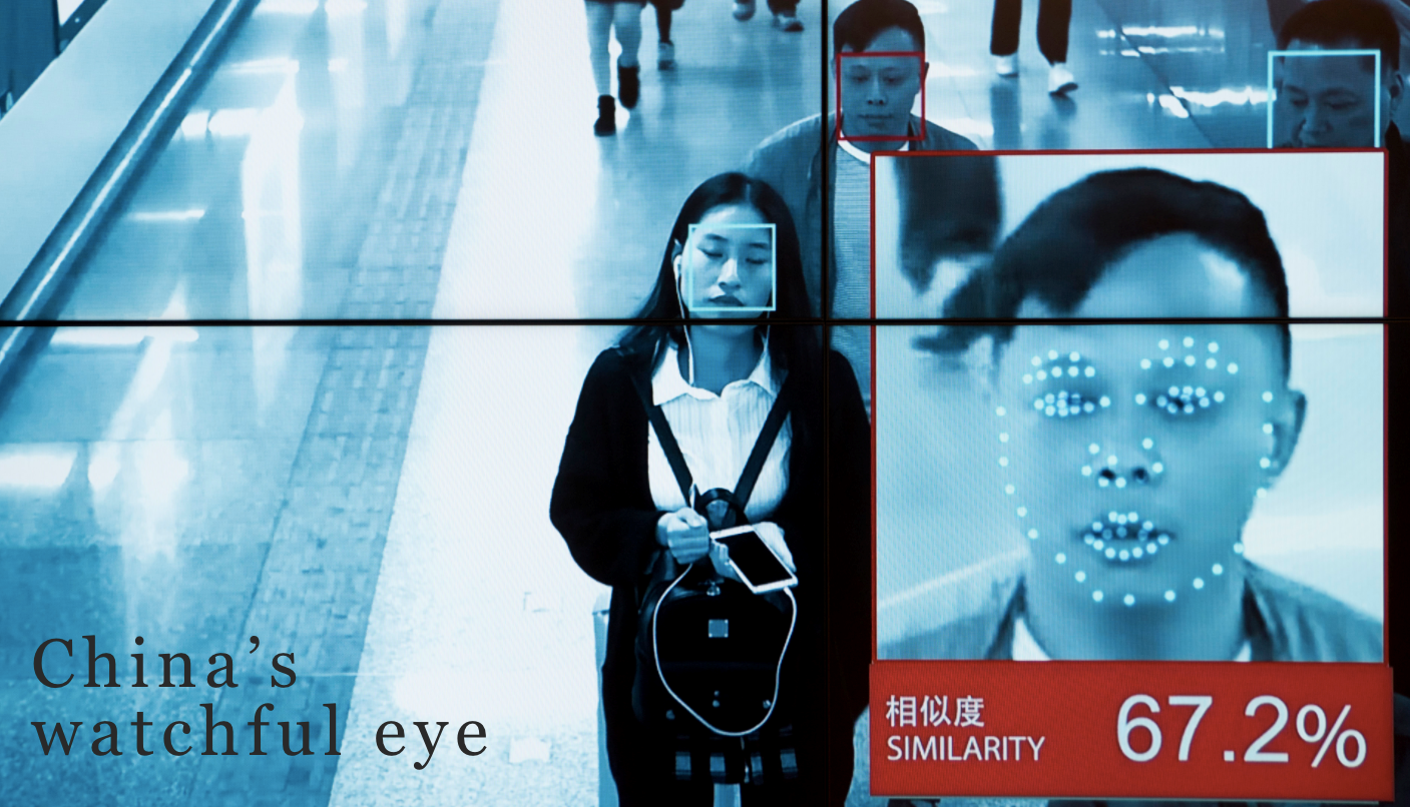
\includegraphics[width=10cm]{china_watchful}
    \end{figure}
    \href{https://www.washingtonpost.com/news/world/wp/2018/01/07/feature/in-china-facial-recognition-is-sharp-end-of-a-drive-for-total-surveillance/?noredirect=on\&utm\_term=.152c95a75d69}{Beijing bets on facial recognition in a big drive for total surveillance} --- Washington Post, 1/8/2018
    \vfill
    \scriptsize{Source: Lazebnik}
\end{frame}

\begin{frame}{Recognition: General Categories}
    \begin{figure}[ht]
        \centering
        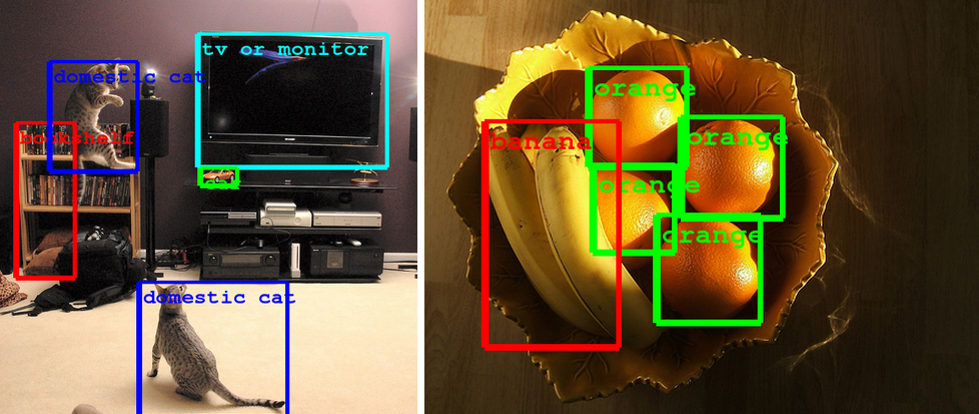
\includegraphics[width=7cm]{general_cat_1.png}
        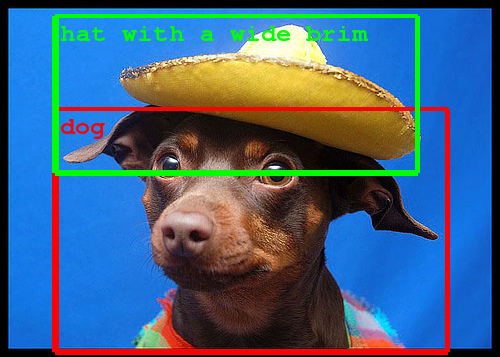
\includegraphics[width=3cm]{general_cat_2.png}
    \end{figure}
    \href{https://bits.blogs.nytimes.com/2014/08/18/computer-eyesight-gets-a-lot-more-accurate/}{Computer Eyesight Gets a Lot More Accurate}, NY Times Bits blog, August 18, 2014
    \href{https://ai.googleblog.com/2014/09/building-deeper-understanding-of-images.html}{Building A Deeper Understanding of Images}, Google Research Blog, September 5, 2014
    \vfill
    \scriptsize{Source: Lazebnik}
\end{frame}


\begin{frame}[fragile]{ImageNet Challenge}

    \begin{tikzpicture}
        \begin{filecontents*}{ilsvrc.dat}
        year,       top5acc,    layers, label
        10,         28.2,       1,
        11,         25.5,       1,
        12,         16.4,       8,      AlexNet
        13,         11.7,        8,
        14,         7.4,         16,      VGG16
        14,         6.7,         22,     GoogleNet
        15,         3.57,        152,    ResNet
        16,         2.99,           ,   Trimps-Soushen
        17,         2.25,           154, SENet
       \end{filecontents*}
        \pgfplotsset{set layers}
        \begin{axis}
        [
            scale only axis,
            ybar,
            nodes near coords,
            axis y line*=left,
            xlabel=Year,
            ylabel style = {align=center},
            ylabel={Top-5 error (percent) \ref{pgfplots:plot1}},
            ]
            \addplot [pattern=horizontal lines light blue] table[x=year, y=top5acc, meta=label, col sep=comma] {ilsvrc.dat};
            \label{pgfplots:plot1}
        \end{axis}

        \begin{axis}
        [
            scale only axis,
            axis y line*=right,
            axis x line=none,
            nodes near coords,
            y label style={at={(1.3,0.5)}},
            ylabel={No. layers \ref{pgfplots:plot2}}
        ]
            \addplot [red] table[x=year, y=layers, col sep=comma] {ilsvrc.dat};
            \node[rotate=90] at (axis cs:12,120) {\scriptsize AlexNet};
            \node[rotate=90] at (axis cs:14,120) {\scriptsize VGG16};
            \node[rotate=90] at (axis cs:14,0) {\scriptsize GoogLeNet};
            \node[rotate=90] at (axis cs:15,120) {\scriptsize ResNet};
            \node[rotate=90] at (axis cs:17,120) {\scriptsize SENet};
            \label{pgfplots:plot2}
        \end{axis}


    \end{tikzpicture}
    \href{http://image-net.org/challenges/LSVRC/}{ILSVRC}
\end{frame}



\begin{frame}{Bengio, Hinton and LeCun Win the Turing Award}
    \begin{figure}[ht]
        \centering
        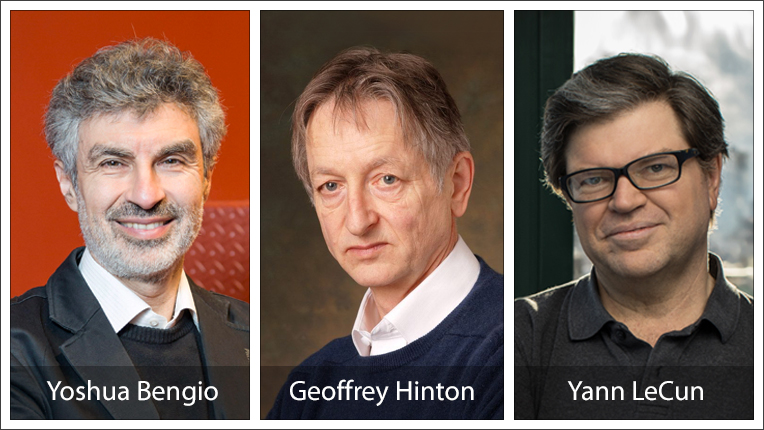
\includegraphics[width=10cm]{turing_2018.jpg}
    \end{figure}
    \href{https://www.acm.org/media-center/2019/march/turing-award-2018}{Fathers of the Deep Learning Revolution Receive ACM A. M. Turing Award}
\end{frame}



\begin{frame}{Recognition: Instance Segmentation}
    \begin{figure}[ht]
      \centering
      \begin{subfigure}[b]{0.5\linewidth}
        \centering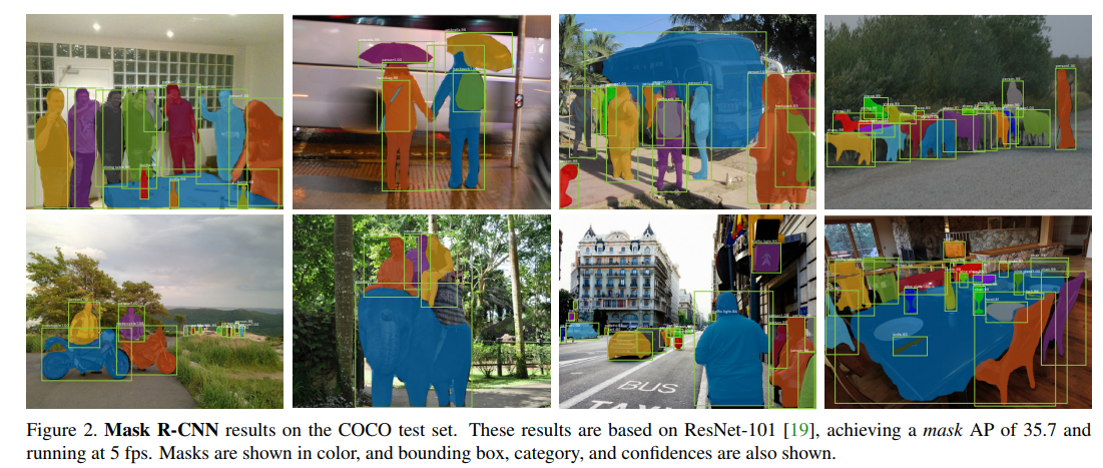
\includegraphics[width=200pt]{mask_rcnn_2}
        \caption{}\label{sf:digital_cameras}
      \end{subfigure}%
      \begin{subfigure}[b]{0.5\linewidth}
        \centering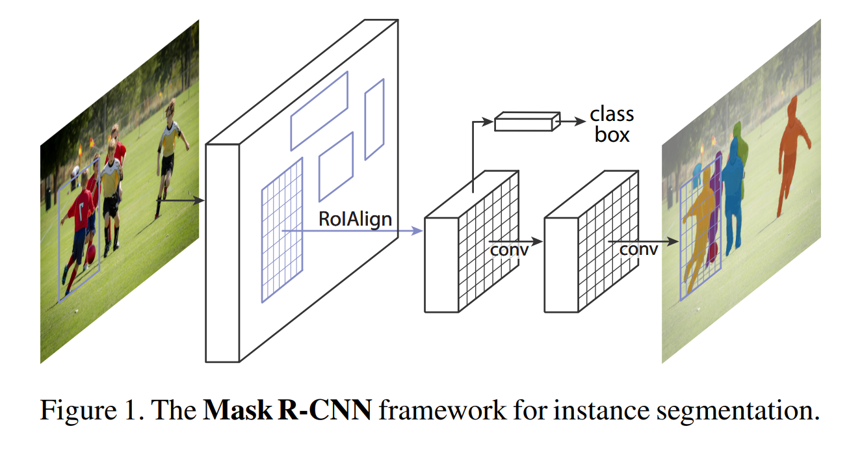
\includegraphics[width=200pt]{mask_rcnn_3}
        \caption{}\label{sf:fr_software}
      \end{subfigure}
      \caption{}
    \end{figure}
    K. He, G. Gkioxari, P. Doll{\'a}r, and R. Girshick, ``Mask R-CNN,'' in IEEE International Conference on Computer Vision, Venice, Italy, 2017, pp. 2980--2988.
\end{frame}



\begin{frame}{Image Generation}
    \begin{figure}[ht]
      \centering
        \centering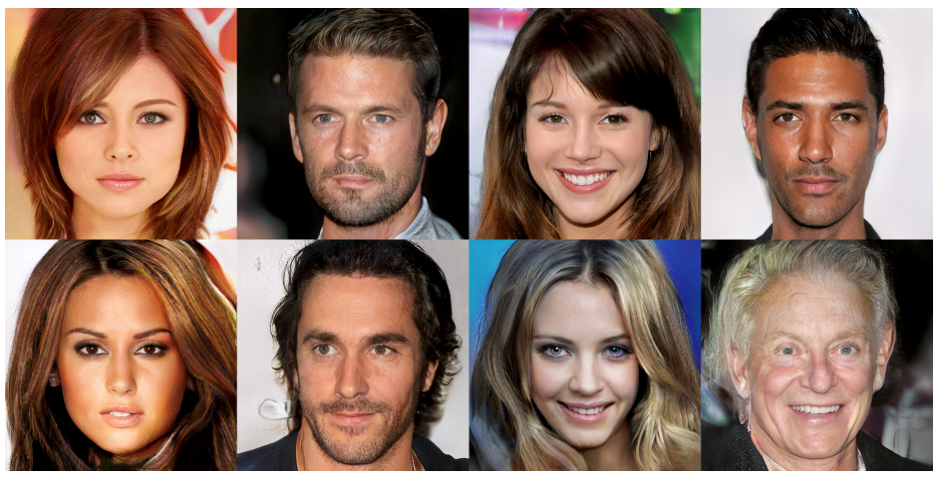
\includegraphics[width=200pt]{growing_gans.png}
    \end{figure}
    T. Karras, T. Aila, S. Laine, and J. Lehtinen, \href{https://www.youtube.com/watch?v=G06dEcZ-QTg&feature=youtu.be}{Progressive Growing of GANs for Improved Quality}, Stability, and Variation, ICLR 2018.
    \vfill
    \scriptsize{Source: Lazebnik}
\end{frame}

\begin{frame}{Image Generation}
    \begin{figure}[ht]
      \centering
        \centering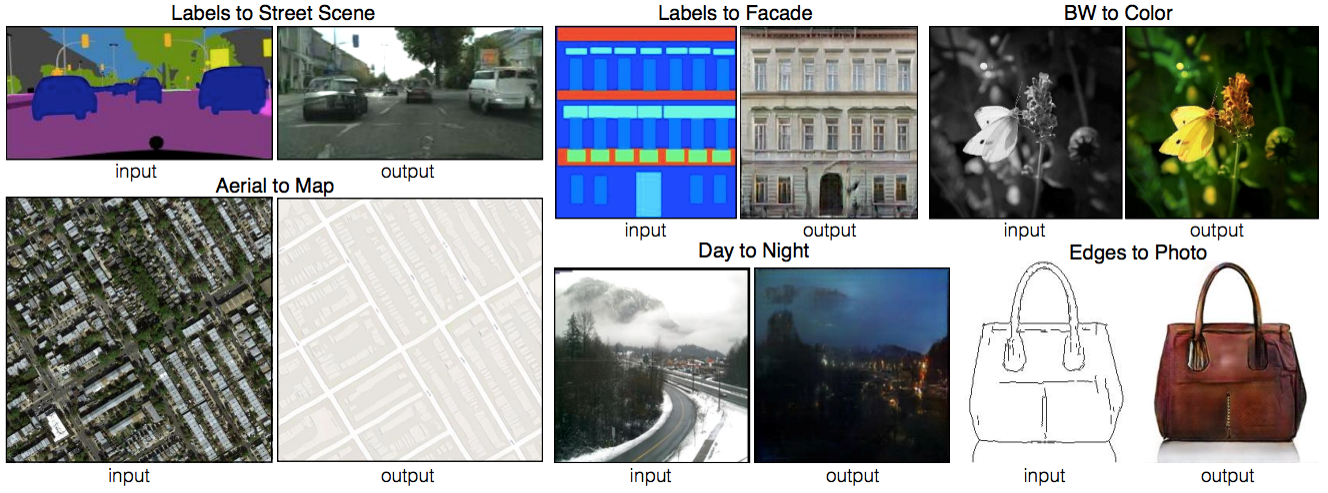
\includegraphics[width=200pt]{image2image.png}
    \end{figure}
    P. Isola, J.-Y. Zhu, T. Zhou, A. Efros, Image-to-Image Translation with Conditional Adversarial Networks, CVPR 2017.
    \vfill
    \scriptsize{Source: Lazebnik}
\end{frame}


\begin{frame}{Deep Video Portraits (DeepFakes)}
    \begin{figure}[ht]
      \centering
        \centering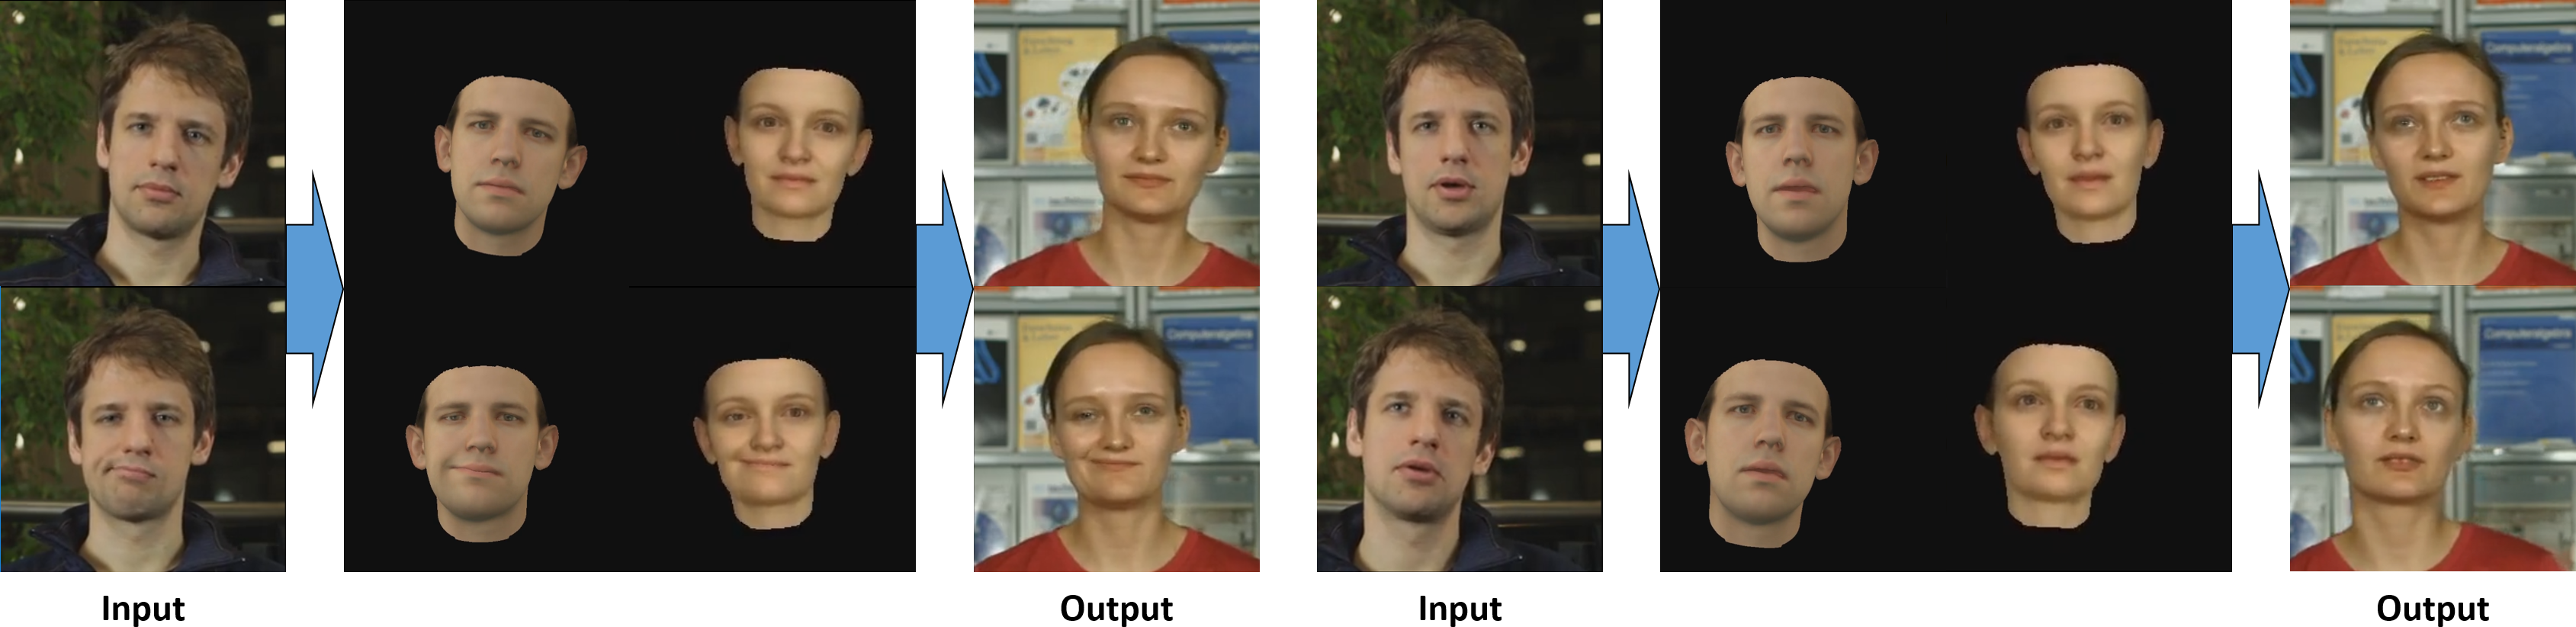
\includegraphics[width=200pt]{deepfakes.png}
    \end{figure}
    Kim, H. and Garrido, P. and Tewari, A. and Xu, W. and Thies, J. and Nie{\ss}ner, N. and P{\'e}rez, P. and Richardt, C. and Zollh{\"o}fer, M. and Theobalt, C. \href{https://web.stanford.edu/~zollhoef/papers/SG2018_DeepVideo/page.html}{Deep Video Portraits}, Siggraph 2018.
    \vfill
    \scriptsize{Source: Lazebnik}
\end{frame}


\begin{frame}{Origins of Computer Vision}
    \begin{figure}[ht]
      \centering
      \begin{subfigure}[b]{0.45\linewidth}
        \centering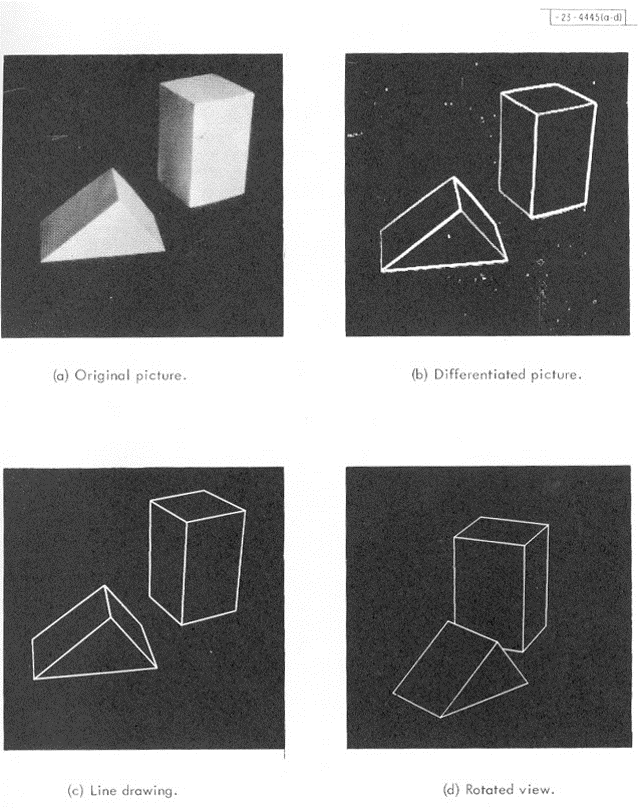
\includegraphics[width=150pt]{roberts}
        \caption{Machine perception of three-dimensional solids by Lawrence G. Roberts, MIT 1937}\label{sf:roberts}
      \end{subfigure}%
      \begin{subfigure}[b]{0.5\linewidth}
        \centering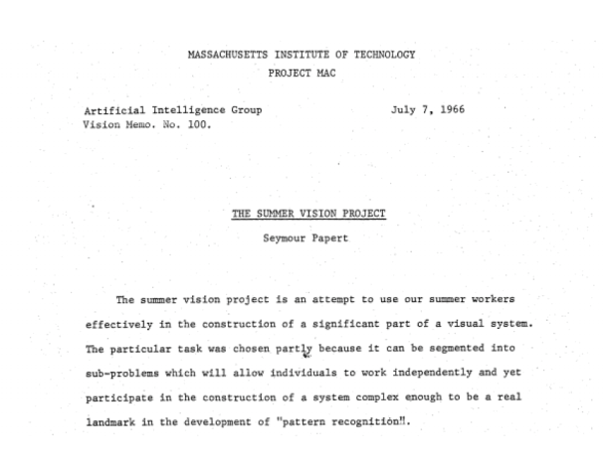
\includegraphics[width=200pt]{papert}
        \caption{The Summer Vision Project at MIT, 1966.}\label{sf:papert}
      \end{subfigure}
      \caption{}
    \end{figure}
    \vfill
    \scriptsize{Source: Lazebnik}
\end{frame}

\begin{frame}{Connections to Other Disciplines}
    \begin{center}
    \begin{tikzpicture}[scale=0.6]
    \tikzset{every node/.append style={scale=0.65}}
      \path[mindmap,concept color=black,text=white]
        node[concept] { Computer vision}
        [clockwise from=0]
        child[concept color=green!50!black] {
          node[concept] { Artificial Intelligence}
        }
        child[concept color=blue] { node[concept] { Machine Learning
    } }
        child[concept color=red] { node[concept] { Cognitive science Neuroscience
    } }
        child[concept color=orange] { node[concept] { Image Processing
    } }
        child[concept color=purple] { node[concept] { Computer Graphics
    } }
        child[concept color=brown] { node[concept] { Robotics} };
    \end{tikzpicture}
\end{center}
    \vfill
    \scriptsize{Source: Lazebnik}
\end{frame}


\begin{frame}{Module Outline}
    \begin{enumerate}
        \item Early vision
            \begin{enumerate}
                \item Point operations, liner filtering, and edge detection
                \item Cameras, light, and color
                \item Feature extraction
                \item Optical flow
                \item Morphological processing
                \item Frequency domain processing.
            \end{enumerate}
        \item Mid-level vinson
            \begin{enumerate}
                \item Fitting: least squares, total squares, RANSAC, Hough lines
                \item Alignment
                \item Image stitching
            \end{enumerate}
        \item Multiple-View Geometry
            \begin{enumerate}
                \item Epipolar geometry
                \item Two-view stereo
                \item Structure from motion
            \end{enumerate}
        \item Recognition
            \begin{enumerate}
                \item Basic classification
                 \item Object detection
                 \item Segmentation
                 \item Deep learning in classification and detection
            \end{enumerate}
    \end{enumerate}
\end{frame}
